\chapter{適用例}\label{cha:Indication}
本章では、本研究で提案した手法が正しく動作することを確認する。
適用例として、本ツールを適用する帳票画像を、図\ref{fig:indication_original}に示す。

\begin{figure}[t]
    \begin{center}
        \fbox{
            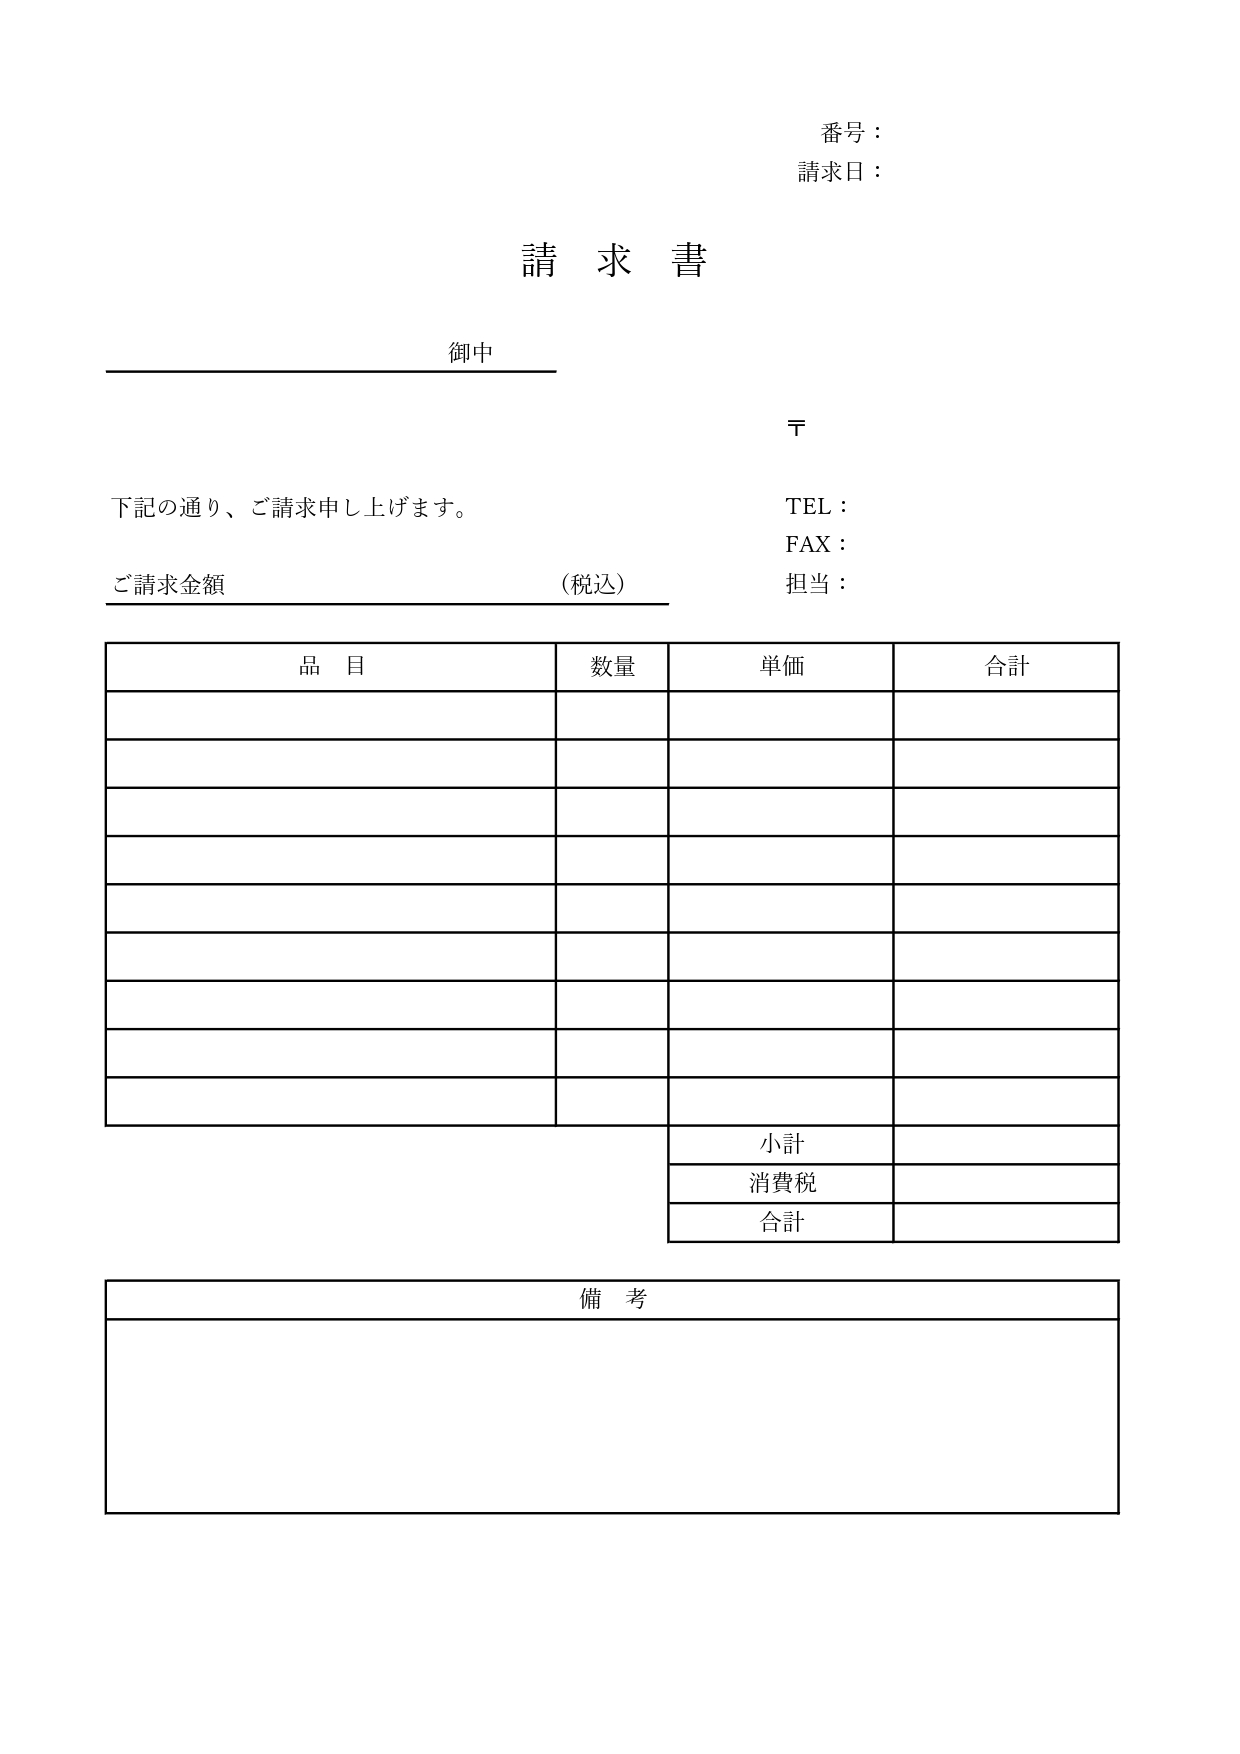
\includegraphics[width=15cm]{image/05-indication/indication_original.jpg}
        }
        \caption{本ツールを適用する帳票画像}
        \label{fig:indication_original}
    \end{center}
\end{figure}

図\ref{fig:indication_original}に対して、本ツールを適用し、出力であるJSONファイルと、矩形領域強調画像と下線部領域強調画像の2枚の領域強調画像を確認する。
具体的には、矩形領域強調画像と、JSONファイルのrects\_data配列を参照し、矩形領域の出力結果を確認する。
同様に、下線部領域強調画像と、JSONファイル内のunderlines\_data配列を参照し、下線部領域の出力結果を確認する。

図\ref{fig:indication_original}に対して、本ツールを適用し、出力したJSONファイルのうち、rects\_data配列の一部を、図\ref{fig:rects_data_json}に示す。
図\ref{fig:rects_data_json}のJSONファイルと同時に出力した2枚の領域強調画像のうち、矩形領域を強調した画像の一部を、図\ref{fig:highlighted_rects_part}に示す。

\lstset{language=}
\begin{figure}[t]
    \begin{lstlisting}
        {
            "id": 4,
            "label": "string",
            "coords": {
                "top_left": {
                    "x": 275,
                    "y": 817
                },
                "buttom_left": {
                    "x": 275,
                    "y": 903
                },
                "buttom_right": {
                    "x": 1008,
                    "y": 903
                },
                "top_right": {
                    "x": 1008,
                    "y": 817
                }
            }
        },
        {
            "id": 5,
            "label": "number",
            "coords": {
                "top_left": {
                    "x": 1016,
                    "y": 817
                },
                "buttom_left": {
                    "x": 1016,
                    "y": 903
                },
                "buttom_right": {
                    "x": 1308,
                    "y": 903
                },
                "top_right": {
                    "x": 1308,
                    "y": 817
                }
            }
        },
    \end{lstlisting}
    \caption{rects\_data配列の一部}\label{fig:rects_data_json}
\end{figure}

\begin{figure}[t]
    \begin{center}
        \fbox{
            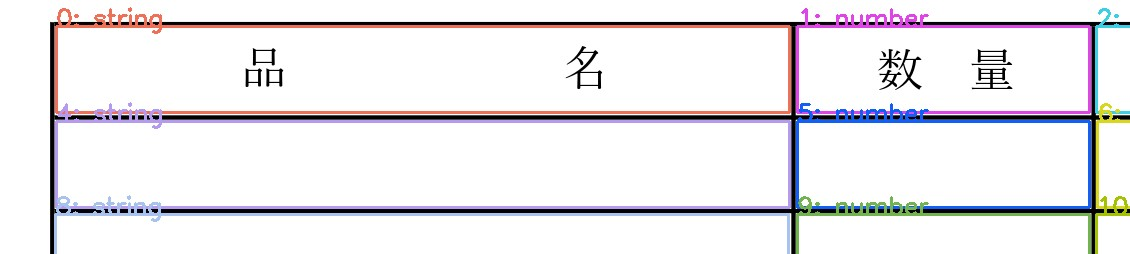
\includegraphics[width=15cm]{image/05-indication/highlighted_rects_part.jpg}
        }
        \caption{矩形領域を強調した画像の一部}
        \label{fig:highlighted_rects_part}
    \end{center}
\end{figure}

また、図\ref{fig:indication_original}に対して、本ツールを適用し、出力したJSONファイルのうち、underline\_data配列の一部を、図\ref{fig:underlines_data_json}に示す。
図\ref{fig:underlines_data_json}のJSONファイルと同時に出力した2枚の下線部強調画像のうち、下線部領域を強調した画像の一部を図\ref{fig:highlighted_underlines_part}に示す。

\lstset{language=}
\begin{figure}[t]
    \begin{lstlisting}
        {
            "id": 0,
            "label": "date",
            "left": {
                "x": 869,
                "y": 354
            },
            "right": {
                "x": 1512,
                "y": 354
            }
        },
        {
            "id": 1,
            "label": "number",
            "left": {
                "x": 1908,
                "y": 355
            },
            "right": {
                "x": 2265,
                "y": 355
            }
        },
    \end{lstlisting}
    \caption{underline\_data配列の一部}\label{fig:underlines_data_json}
\end{figure}

\begin{figure}[t]
    \begin{center}
        \fbox{
            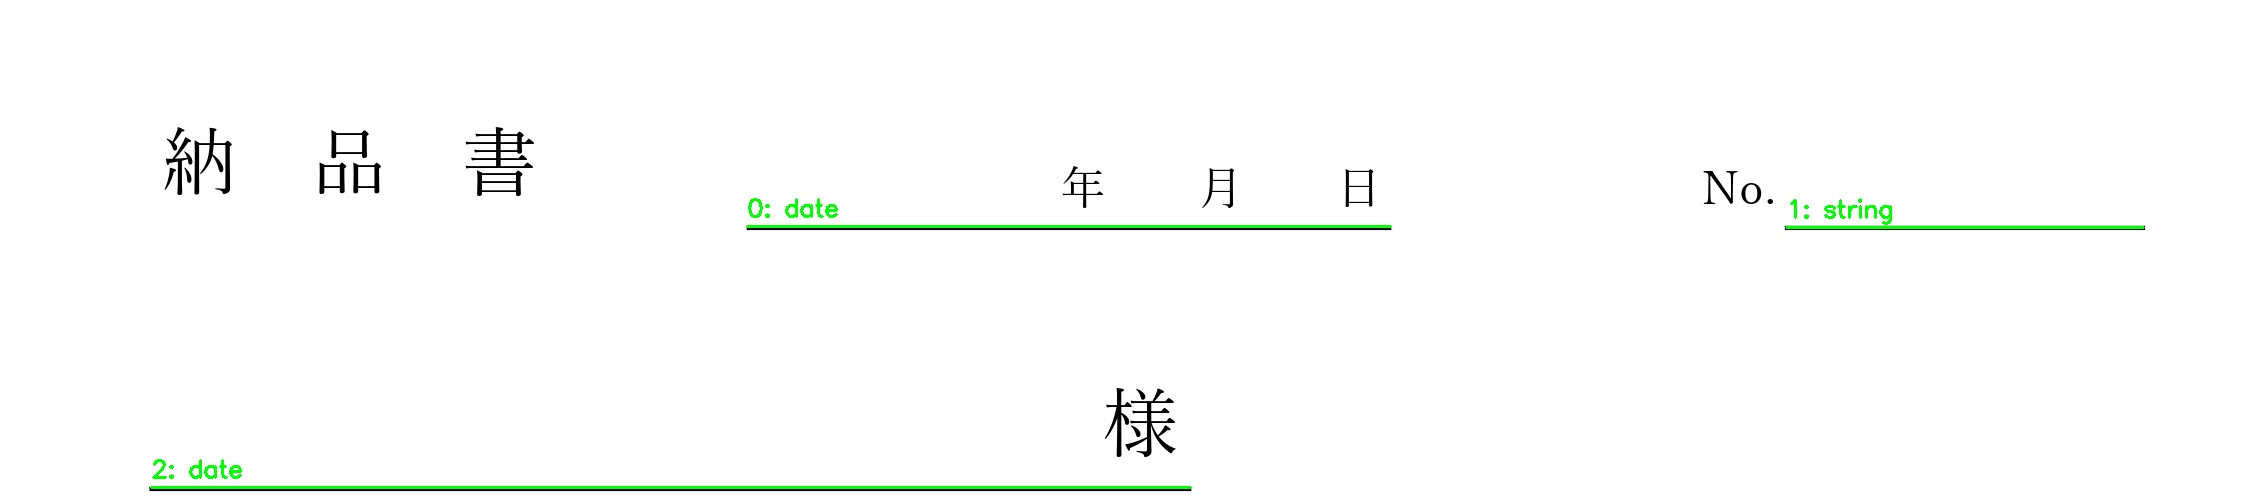
\includegraphics[width=15cm]{image/05-indication/highlighted_underlines_part.jpg}
        }
        \caption{下線部領域を強調した画像の一部}
        \label{fig:highlighted_underlines_part}
    \end{center}
\end{figure}

\section{矩形領域についての出力結果}\label{sec:result_rect}
本節は、矩形領域についての出力結果を確認する。

矩形領域座標については、IoU(Intersection over Union)を用いて、JSONファイルの出力が正しいことを確認する。
IoUは、物体検出において、2つの領域の重なり度合いを表す指標であり、1.0で完全一致、0.0で重なりがないことを示す。

IoUを算出する式を、以下に示す。
なお、一般に、IoUは0.5を閾値として、閾値以上である場合は一致とみなされる\cite{IoU閾値}。

\begin{equation}
    \rm{IoU} = \frac{2つの領域の積集合}{2つの領域の和集合}
\end{equation}

人間が確認したの矩形領域座標と、出力するJSONファイルの矩形領域座標を確認し、IoUを算出する。
図\ref{fig:rects_data_json}より、idキーに対応する値が4である矩形領域座標は、左上頂点のxy座標が(275,817)であり、右下頂点のxy座標が(1008,903)である。
図\ref{fig:highlighted_rects_part}にある4番の矩形領域について、図\ref{fig:indication_original}の画像では、左上頂点のxy座標が(273,816)であり、右下頂点のxy座標が(1009,905)である。
よって、IoUを算出すると、0.96となるため、この矩形領域座標は正しく取得できたと言える。
他の矩形領域に対しても、正しく矩形領域座標を取得していることを確認した。

ラベルについては、JSONファイルの内容と、矩形領域強調画像で描画する番号とラベルが一致するかを確認する。
図\ref{fig:rects_data_json}より、idキーに対応する値は4と5であり、それぞれラベルはstring、numberである。
図\ref{fig:highlighted_rects_part}より、画像内に描画した矩形領域の番号のうち、4番の矩形領域は、「品名」を記入する欄であり、5番の矩形領域は、「数量」を記入する欄であることがわかる。
「品名」、「数量」という記入欄については、文字列(string)、数値(number)が正しいラベルであるため、これら2つの矩形領域については、正しくラベルを割り付けていることを確認できた。
他の矩形領域に対しても、一部を除き、正しくラベルを割り付けていることを確認した。

一部の矩形領域については、本来割り付けるべきラベルとは異なるラベルを誤って割り付けた。
JSONファイルのうち、誤ったラベルを割り付けた矩形領域座標を、図\ref{fig:rects_data_miss_json}に示す。
また、図\ref{fig:rects_data_miss_json}に示した箇所の矩形領域強調画像を、図\ref{fig:highlighted_rects_miss_part}に示す。

\lstset{language=}
\begin{figure}[t]
    \begin{lstlisting}
        {
            "id": 25,
            "label": "string",
            "coords": {
                "top_left": {
                    "x": 1713,
                    "y": 1283
                },
                "buttom_left": {
                    "x": 1713,
                    "y": 1369
                },
                "buttom_right": {
                    "x": 2262,
                    "y": 1369
                },
                "top_right": {
                    "x": 2262,
                    "y": 1283
                }
            }
        },
    \end{lstlisting}
    \caption{誤ったラベルを割り付けた矩形領域座標}\label{fig:rects_data_miss_json}
\end{figure}

\begin{figure}[t]
    \begin{center}
        \fbox{
            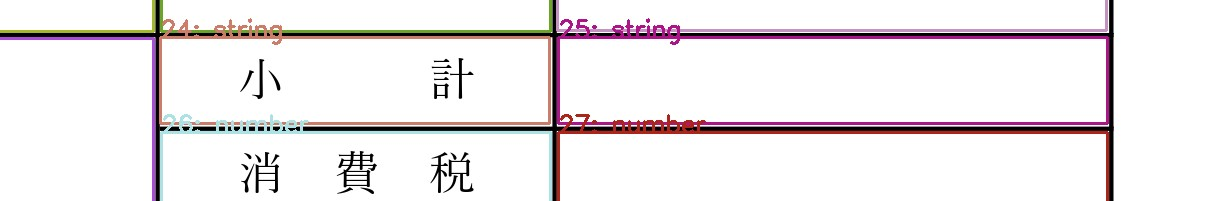
\includegraphics[width=15cm]{image/05-indication/highlighted_rects_miss_part.jpg}
        }
        \caption{図\ref{fig:rects_data_miss_json}の矩形領域を描画した矩形領域強調画像}
        \label{fig:highlighted_rects_miss_part}
    \end{center}
\end{figure}

図\ref{fig:rects_data_miss_json}より、idキーに対応する値が25の矩形領域は、labelキーに対応する値がstringであることがわかる。
図\ref{fig:highlighted_rects_miss_part}より、25番の矩形領域は、「小計」を記入する欄であることがわかる。
本来割り付けるべきラベルは数値(number)であるため、誤ったラベルを割り付けていることがわかる。
これは、「小計」という文字を認識することができなかったためである。

図\ref{fig:indication_original}の画像に対して、認識した文字のバウンディングボックスを描画した画像の一部を、図\ref{fig:OCR_result}に示す。
図\ref{fig:OCR_result}の右にある「小計」については、バウンディングボックスを描画していないため、文字認識に失敗していることがわかる。
また、図\ref{fig:OCR_result}の左にある「備考」の文字について、属性を文字列(string)と推測したことを確認した。
これによって、文字認識を失敗したことによって、認識するべき文字とは別の文字の属性をラベルとして割り付けたことが、誤ったラベルを割り付けた原因であることがわかる。
この問題点については、\ref{sec:problems}節で後述する。

\begin{figure}[t]
    \begin{center}
        \fbox{
            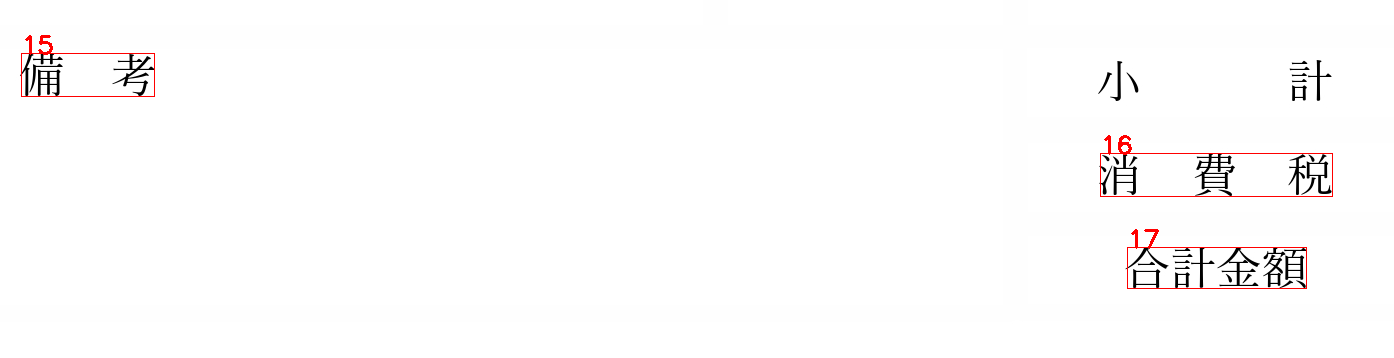
\includegraphics[width=15cm]{image/05-indication/OCR_result.png}
        }
        \caption{図\ref{fig:indication_original}で認識した文字}
        \label{fig:OCR_result}
    \end{center}
\end{figure}

\section{下線部領域についての出力結果}\label{sec:result_underline}
本節は、下線部領域についての出力結果を確認する。

下線部領域座標については、矩形領域座標と同様に、IoUを用いて、JSONファイルの出力が正しいことを確認する。
なお、下線部領域については、高さを3ピクセルとして、IoUを計算する。
人間が確認した下線部領域座標と、出力するJSONファイルの下線部領域座標を確認し、IoUを算出する。
図\ref{fig:underlines_data_json}より、idキーに対応する値が0である下線部領域座標は、左端点のxy座標が(869,354)であり、右端点のxy座標が(1512,354)である。
図\ref{fig:highlighted_underlines_part}にある0番の下線部領域について、図\ref{fig:indication_original}の画像では、左端点のxy座標が(869,354)であり、右端点のxy座標が(1511,354)である。
よって、IoUを算出すると、0.99でとなるため、この下線部領域座標は正しく取得できたと言える。
他の下線部領域に対しても、正しく下線部領域座標を取得していることを確認した。

図\ref{fig:underlines_data_json}より、idキーに対応する値は0と1であり、それぞれラベルはdate、numberとである。
図\ref{fig:highlighted_underlines_part}より、画像内に描画した矩形領域の番号のうち、0番の下線部領域は、「年月日」を記入する欄であり、1番の下線部領域は、「No.」を記入する欄であることがわかる。
「年月日」、「No.」という記入欄については、それぞれ日付(date)、数値(number)が正しいラベルであるため、これら2つの下線部領域については、正しくラベルを割り付けていることを確認できた。
他の下線部領域に対しても、一部を除き、正しくラベルを割り付けていることを確認した。

一部の下線部領域については、本来割り付けるべきラベルとは異なるラベルを誤って割り付けた。
JSONファイルのうち、誤ったラベルを割り付けた下線部領域座標を、図\ref{fig:underlines_data_miss_json}に示す。
図\ref{fig:underlines_data_miss_json}の下線部領域は、図\ref{fig:highlighted_underlines_part}の2番の下線部領域である。

\lstset{language=}
\begin{figure}[t]
    \begin{lstlisting}
        {
            "id": 2,
            "label": "date",
            "left": {
                "x": 273,
                "y": 615
            },
            "right": {
                "x": 1312,
                "y": 615
            }
        },
    \end{lstlisting}
    \caption{誤ってラベルを割り付けた下線部領域}\label{fig:underlines_data_miss_json}
\end{figure}

図\ref{fig:underlines_data_miss_json}より、idキーに対応する値が2の下線部領域は、labelキーに対応する値がdateであることがわかる。
図\ref{fig:highlighted_underlines_part}の左下を確認すると、2番の下線部領域は、右にある「様」という文字から、宛名を記入する欄であることがわかる。
本来割り付けるべきラベルは文字列(string)であるため、誤ったラベルを割り付けていることがわかる。
これは、\ref{subsec:label_link_processing}節で述べたラベルを割り付ける手法では、領域座標の右にある文字の属性を参照しないためである。
この問題点については、\ref{sec:problems}節で後述する。